\documentclass[letterpaper]{article}
\usepackage{geometry}
\usepackage[table,xcdraw]{xcolor}
\geometry{margin=1.1in}
\usepackage[protrusion=true,expansion=true]{microtype}	
\usepackage[boxruled,linesnumbered,vlined,inoutnumbered]{algorithm2e}
\usepackage{amsmath}
\usepackage{amsthm}
\usepackage{amssymb}
\usepackage{mathtools}
\usepackage{mathrsfs}
\usepackage{float}
\usepackage{booktabs}
\usepackage{soul}
\usepackage{natbib}
\usepackage{rotating}
\usepackage{gensymb}
\usepackage{lscape}
\usepackage{array}
\usepackage{makecell}
\renewcommand\theadalign{bc}
\renewcommand\theadfont{\bfseries}
\renewcommand\theadgape{\Gape[4pt]}
\renewcommand\cellgape{\Gape[4pt]}
\usepackage{courier}
\usepackage{lipsum}
\usepackage{graphicx}
\usepackage{subcaption}
\usepackage[space]{grffile}
\usepackage{xcolor}
\definecolor{light-grey}{rgb}{0.9,0.9,0.9}
\definecolor{dark-red}{rgb}{0.4,0.15,0.15}
\definecolor{dark-blue}{rgb}{0,0,0.7}
\usepackage{environ}
\setcounter{tocdepth}{2}
\renewcommand{\contentsname}{Table of Contents}
\usepackage{hyperref}
\hypersetup{
    colorlinks, linkcolor={dark-blue},
    citecolor={dark-blue}, urlcolor={dark-blue}
}

\setlength{\parskip}{1em}
\newcommand{\HIGHLIGHT}[1]{\textcolor{blue}{\textbf{#1}}}
\newcommand{\TODO}[1]{\textcolor{red}{\textbf{#1}}}

\begin{document}
%-----------------
%	Homework 4
%-----------------
\newpage
\begin{center}
    \begin{Large}
    COMPSCI 589 Final Project - Spring 2025
    \end{Large}
    \\
    \HIGHLIGHT{Due May 09, 2025, 11:59pm Eastern Time}
\end{center}
\addcontentsline{toc}{subsection}{\textbf{Final Project}}



\vspace{0.25in}
\section{The Hand-Written Digits Recognition Dataset}
\subsection{Neural Network}
\begin{table}[H]
  \centering
  \caption{Performance on \texttt{digits}}
  \begin{tabular}{l r r r r r}
    \toprule
    Architecture      & $\lambda$ & LR     & Batch & Accuracy & F1-score \\
    \midrule
    \texttt{[64,64]}     & 0.0000    & 0.0030 & 100   & 0.9389   & 0.9373   \\
    \texttt{[64,64]}     & 0.0000    & 0.0070 & 100   & 0.9611   & 0.9604   \\
    \texttt{[64,64]}     & 0.0001    & 0.0030 & 100   & 0.9361   & 0.9334   \\
    \texttt{[64,64]}     & 0.0001    & 0.0070 & 100   & 0.9500   & 0.9494   \\
    \addlinespace
    \texttt{[64,64,64]}   & 0.0000    & 0.0030 & 100   & 0.9528   & 0.9521   \\
    \texttt{[64,64,64]}   & 0.0000    & 0.0070 & 100   & 0.9694   & 0.9687   \\
    \texttt{[64,64,64]}   & 0.0001    & 0.0030 & 100   & 0.9778   & 0.9776   \\
    \texttt{[64,64,64]}   & 0.0001    & 0.0070 & 100   & 0.9722   & 0.9717   \\
    \addlinespace
    \texttt{[128,64,32]}  & 0.0000    & 0.0030 & 100   & 0.9722   & 0.9718   \\
    \texttt{[128,64,32]}  & 0.0000    & 0.0070 & 100   & 0.9806   & 0.9803   \\
    \texttt{[128,64,32]}  & 0.0001    & 0.0030 & 100   & 0.9806   & 0.9803   \\
    \texttt{[128,64,32]}  & 0.0001    & 0.0070 & 100   & 0.9778   & 0.9775   \\
    \bottomrule
  \end{tabular}
\end{table}
$\\$
The best hyperparameter setting for a neural network on the Digits dataset is an architecture of decreasing hidden dimensions ([128, 64, 32]) with low L2 regularization (reg=0.0001), a small learning rate (lr=0.003), and a normal batch size (bs=100). What made this dataset especially challenging to work with was the fact that it was image classification rather than classification using tabular data. Due to semantic differences, images can differ for many reasons from lighting to occlusion, while representing the same semantic object. To overcome this, we designed a specific architecture containing 3 hidden layers of decreasing size that allows for progressively passing high-dimensional representations, like that of images, through the network into more compact feature spaces. The larger layers (128 neurons) capture the general features of the inputs, like shape, while the smaller layers (32 neurons) capture the specific features of the inputs for classification. While the same architecture yielded the same evaluation metrics for having no regularization and a learning rate of 0.007 as well as having a regularization strength of 0.0001 and a learning rate of 0.003, ultimately, we decided that the low regularization paired with the small learning rate is generally more stable and robust in practice. 
\begin{figure}[H]
  \centering
  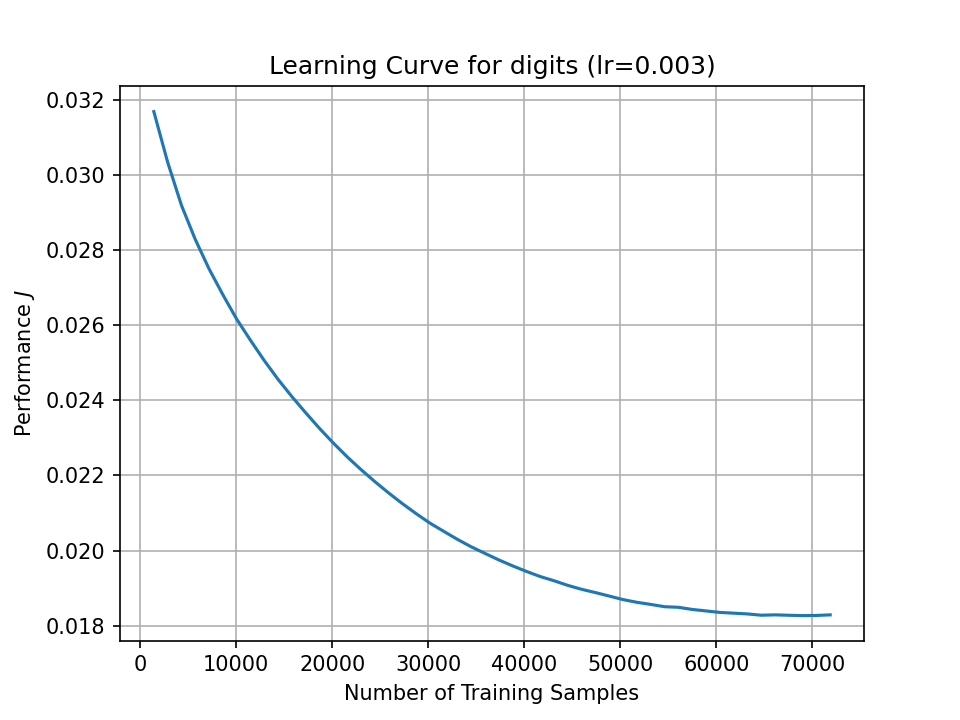
\includegraphics[width=0.8\textwidth]{learning_curves/lc_digits.png}
  \caption{Learning Curve for \texttt{digits} dataset: 3 hidden layers of size [128,\,64,\,32], regularization $\lambda=0.0001$, learning rate lr$=0.003$, batch size bs = 100.}
  \label{fig:lc-digits}
\end{figure}
$\\$
Figure 1 shows a smooth, monotonic descent with stable convergence for the cost J. The curve appears to cut off around the point of diminishing returns, which is highly favorable. Some reasons as to why the neural network's convergence of J was so smooth may be due to its excellent abilities to capture high-level features in its early layers when there are a large number of neurons, allowing for later layers to pick up on fine-grained details. 
\newpage
\subsection{}
% Your Analysis Goes Here

\newpage
\section{The Oxford Parkinson’s Disease Detection Dataset}
\subsection{Neural Network}
\begin{table}[H]
  \centering
  \caption{Performance on \texttt{parkinsons.csv}}
  \begin{tabular}{l r r r r r}
    \toprule
    Architecture      & $\lambda$ & LR     & Batch & Accuracy & F1-score \\
    \midrule
    \texttt{[16,16,16]}  & 0.0008    & 0.0010 & 8     & 0.8718   & 0.7937   \\
    \texttt{[16,16,16]}  & 0.0008    & 0.0015 & 8     & 0.7436   & 0.4265   \\
    \texttt{[16,16,16]}  & 0.0007    & 0.0010 & 8     & 0.7692   & 0.5237   \\
    \texttt{[16,16,16]}  & 0.0007    & 0.0015 & 8     & 0.8718   & 0.7937   \\
    \addlinespace
    \texttt{[32,32,32]}  & 0.0008    & 0.0010 & 8     & 0.8205   & 0.7367   \\
    \texttt{[32,32,32]}  & 0.0008    & 0.0015 & 8     & 0.8462   & 0.7641   \\
    \texttt{[32,32,32]}  & 0.0007    & 0.0010 & 8     & 0.8718   & 0.7937   \\
    \texttt{[32,32,32]}  & 0.0007    & 0.0015 & 8     & 0.8718   & 0.8120   \\
    \addlinespace
    \texttt{[64,64,64]}  & 0.0008    & 0.0010 & 8     & 0.8718   & 0.8120   \\
    \texttt{[64,64,64]}  & 0.0008    & 0.0015 & 8     & 0.8718   & 0.7937   \\
    \texttt{[64,64,64]}  & 0.0007    & 0.0010 & 8     & 0.8718   & 0.7937   \\
    \texttt{[64,64,64]}  & 0.0007    & 0.0015 & 8     & 0.8974   & 0.8427   \\
    \bottomrule
  \end{tabular}
\end{table}
$\\$
The best hyperparameter setting for a neural network on the Oxford Parkinson’s dataset is an architecture of three hidden layers ([64, 64, 64]) with moderate L2 regularization ($\lambda$ = 0.0007), a standard learning rate (lr = 0.0015), and a small batch size (bs = 8). Using three layers of 64 units helps balance between model complexity and performance. Rather than capturing more feature representation from the training sets and risking overfitting, the simple width and depth of the network allow for easy convergence. The moderate regularization strength $\lambda$ = 0.0007 was strong enough to prevent overfitting to the small training set, and the learning rate lr = 0.0015 was stable but provided sufficiently rapid convergence. 

$\\$
The Parkinson's dataset was particularly challenging due to the number of features. The common "curse of dimensionality" holds especially when there are a small number of data points. Specifically, as the feature dimensions increase, the input volume increases as well - but as the number of data points decreases, the sparsity increases, limiting generalization due to overfitting.
\begin{figure}[H]
  \centering
  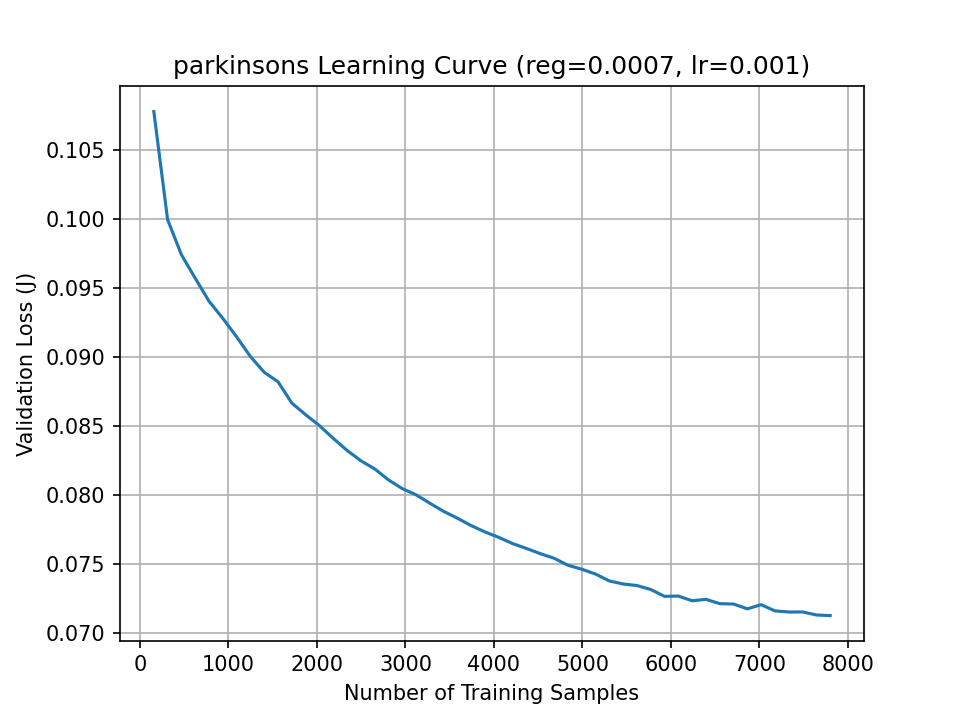
\includegraphics[width=0.8\textwidth]{learning_curves/lc_parkinsons.png}
  \caption{Learning Curve for \texttt{parkinsons} dataset: 3 hidden layers of size [64,\,64,\,64], L2 regularization $\lambda=0.0007$, learning rate lr$=0.0015$, batch size bs= 8.}
  \label{fig:lc-parkinsons}
\end{figure}
$\\$
Figure 3 shows a sharp drop in the cost J initially during the first few epochs, then a more gradual decline as the network continues to capture the fine-grained details within the features during later epochs. The small batch size introduces a bit of noise in a few epochs, shown by the curve's small oscillations, but this instability can prevent the model from converging at local minima and improve generalization. Furthermore, smaller batch sizes produce more weight updates per epoch, accelerating convergence. This acceleration was a necessity due to the limited number of data points in the dataset, limiting the amount of weight updates had the batch size been any larger, potentially preventing the network from converging. The curve demonstrates good convergence without any signs of overfitting, validating our choice in the hyperparameters. 

\newpage
\subsection{}
% Your Analysis Goes Here

\newpage
\section{The Rice Grains Dataset}
\subsection{Neural Network}
\begin{table}[H]
  \centering
  \caption{Performance on \texttt{rice.csv}}
  \begin{tabular}{l r r r r r}
    \toprule
    Architecture      & $\lambda$ & LR     & Batch & Accuracy & F1-score \\
    \midrule
    \texttt{[32,32]}     & 0.0000    & 0.0030 & 100   & 0.9423   & 0.9406   \\
    \texttt{[32,32]}     & 0.0000    & 0.0070 & 100   & 0.9409   & 0.9397   \\
    \texttt{[32,32]}     & 0.0010    & 0.0030 & 100   & 0.9436   & 0.9422   \\
    \texttt{[32,32]}     & 0.0010    & 0.0070 & 100   & 0.9396   & 0.9378   \\
    \addlinespace
    \texttt{[64,64]}     & 0.0000    & 0.0030 & 100   & 0.9449   & 0.9436   \\
    \texttt{[64,64]}     & 0.0000    & 0.0070 & 100   & 0.9423   & 0.9407   \\
    \texttt{[64,64]}     & 0.0010    & 0.0030 & 100   & 0.9423   & 0.9408   \\
    \texttt{[64,64]}     & 0.0010    & 0.0070 & 100   & 0.9423   & 0.9409   \\
    \addlinespace
    \texttt{[64,64,64]}  & 0.0000    & 0.0030 & 100   & 0.9278   & 0.9250   \\
    \texttt{[64,64,64]}  & 0.0000    & 0.0070 & 100   & 0.9383   & 0.9371   \\
    \texttt{[64,64,64]}  & 0.0010    & 0.0030 & 100   & 0.9423   & 0.9409   \\
    \texttt{[64,64,64]}  & 0.0010    & 0.0070 & 100   & 0.9449   & 0.9435   \\
    \bottomrule
  \end{tabular}
\end{table}
$\\$
The best hyperparameter setting for a neural network on the Rice Grains dataset is an architecture of two hidden layers ([64, 64]) with no L2 regularization ($\lambda = 0.0$), a moderate learning rate (lr$= 0.003$), and a moderate batch size (bs$= 100$). While the dataset did not provide any specific challenges regarding the features and data types themselves (being a small amount and all numeric), it did provide a challenge due to its immense number of data points. Using two layers of 64 neurons balances complexity and performance best on this dataset, and excluding regularization did not lead to overfitting, likely because the dataset is large enough and the model capacity is well fitted to classification with a smaller number of features. The learning rate lr$=0.003$ allowed for easy convergence.
\begin{figure}[H]
  \centering
  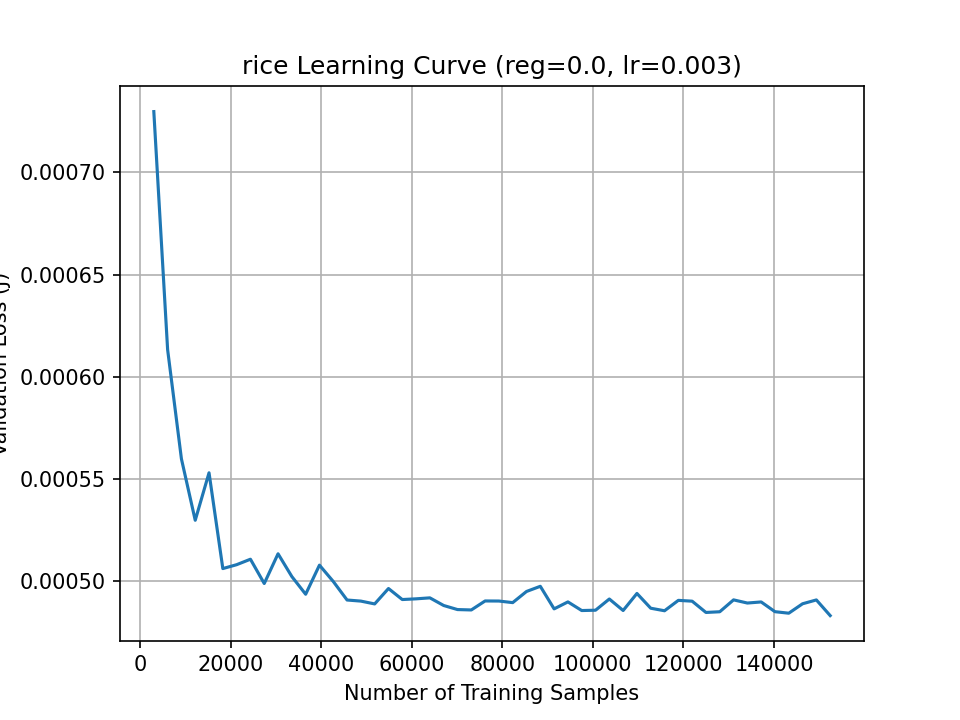
\includegraphics[width=0.8\textwidth]{learning_curves/lc_rice.png}
  \caption{Learning Curve for \texttt{rice} dataset: 2 hidden layers of size [64,\,64], no regularization ($\lambda=0$), learning rate lr$=0.003$, batch size = 100.}
  \label{fig:lc-rice}
\end{figure}
$\\$
Figure 5 shows an initial steep decline in the cost $J$ during the first few epochs. This is followed by a relatively unstable, plateaued descent, indicating that the training of the network’s weights was not robust to fine-grained variations within the classes. The curve has pronounced oscillations that demonstrate that the gradient calculations provided overestimated updates; however, the plateau ultimately shows convergence without overfitting.

\newpage
\subsection{}
% Your Analysis Goes Here

\newpage
\section{The Credit Approval Dataset}
\subsection{Neural Network}
\begin{table}[H]
  \centering
  \caption{Performance on \texttt{credit\_approval.csv}}
  \begin{tabular}{l r r r r r}
    \toprule
    Architecture      & $\lambda$ & LR     & Batch & Accuracy & F1-score \\
    \midrule
    \texttt{[64,64,64]}   & 0.0008    & 0.0010 & 16    & 0.9084   & 0.9077   \\
    \texttt{[64,64,64]}   & 0.0008    & 0.0015 & 16    & 0.9160   & 0.9157   \\
    \texttt{[64,64,64]}   & 0.0009    & 0.0010 & 16    & 0.8931   & 0.8924   \\
    \texttt{[64,64,64]}   & 0.0009    & 0.0015 & 16    & 0.9008   & 0.9004   \\
    \addlinespace
    \texttt{[128,128,128]} & 0.0008    & 0.0010 & 16    & 0.9084   & 0.9081   \\
    \texttt{[128,128,128]} & 0.0008    & 0.0015 & 16    & 0.8931   & 0.8928   \\
    \texttt{[128,128,128]} & 0.0009    & 0.0010 & 16    & 0.9084   & 0.9080   \\
    \texttt{[128,128,128]} & 0.0009    & 0.0015 & 16    & 0.9160   & 0.9155   \\
    \addlinespace
    \texttt{[256,256,256]} & 0.0008    & 0.0010 & 16    & 0.9160   & 0.9155   \\
    \texttt{[256,256,256]} & 0.0008    & 0.0015 & 16    & 0.9084   & 0.9080   \\
    \texttt{[256,256,256]} & 0.0009    & 0.0010 & 16    & 0.9084   & 0.9080   \\
    \texttt{[256,256,256]} & 0.0009    & 0.0015 & 16    & 0.9008   & 0.9004   \\
    \bottomrule
  \end{tabular}
\end{table}
$\\$
The best hyperparameter setting for a neural network on the Credit Approval dataset is an architecture of three hidden layers ([64, 64, 64]) with a small L2 regularization strength ($\lambda = 0.0008$), a moderate learning rate (lr$ = 0.001$), and a small batch size (bs = 16). 
One of the challenges of this dataset was the fact that it had so many categorical features that increased the volume of the input space as well as sparsity. Using three layers of 64 neurons balances model complexity with performance on this small, noisy tabular dataset. The small regularization $\lambda = 0.0008$ allows for weight updates to improve generalization without under-fitting, while the learning rate $\eta = 0.001$ ensures that the model converges to a proper minima. The small batch size of 16 allows for more frequent weight updates per epoch, ultimately accelerating convergence and escape shallow local minima.
\begin{figure}[H]
\centering
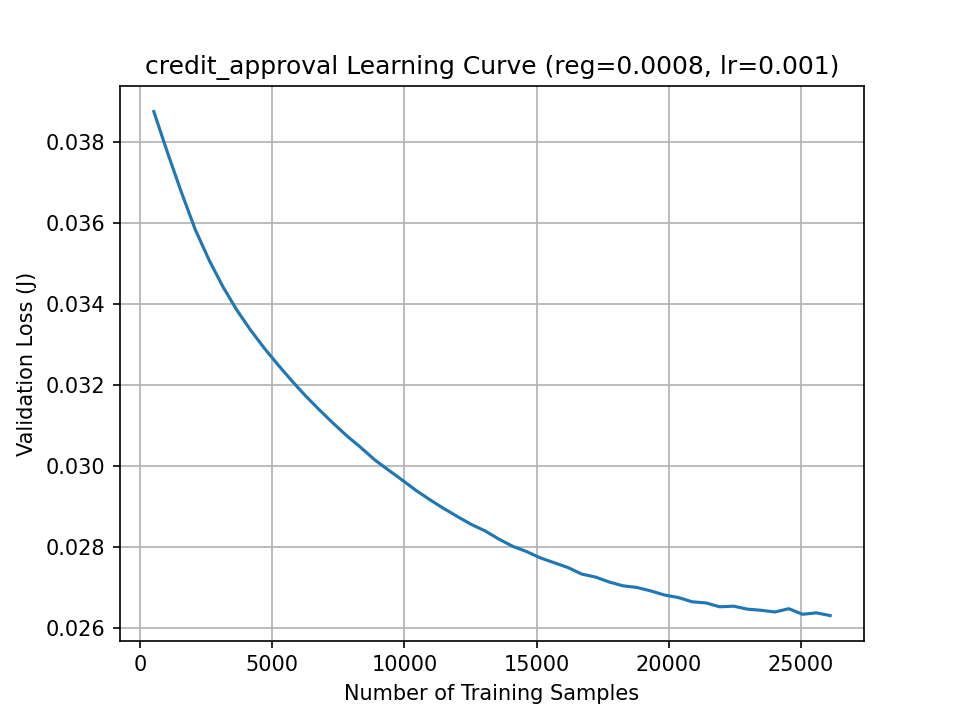
\includegraphics[width=0.8\textwidth]{learning_curves/lc_approval.png}
\caption{Learning Curve for \texttt{credit\_approval} dataset: 3 hidden layers of size [64,64,64], L2 regularization $\lambda=0.0008$, learning rate lr$=0.0015$, batch size = 16.}
\label{fig:lc-credit}
\end{figure}
$\\$
Figure 7 shows a smooth initial descent in the cost J, followed by a slower descent at later epochs. The small oscillations at later epochs are most likely due to the low batch size, providing noise that prevents early convergence. The flat plateau at the later epochs indicate good generalization.

\newpage
\subsection{}
% Your Analysis Goes Here

\newpage
\section{Summary}
\begin{table}[H]
\begin{tabular}{|
>{\columncolor[HTML]{FFFFFF}}l |
>{\columncolor[HTML]{FFFFFF}}l |
>{\columncolor[HTML]{FFFFFF}}l |
>{\columncolor[HTML]{FFFFFF}}l |
>{\columncolor[HTML]{FFFFFF}}l |}
\hline
               & Digits                                                                & Parkinson's                                                           & Rice                                                                  & Credit\_Approval                                                     \\ \hline
Neural Network & \begin{tabular}[c]{@{}l@{}}Acc      F1\\ 0.9806 | 0.9803\end{tabular} & \begin{tabular}[c]{@{}l@{}}Acc      F1\\ 0.8974 | 0.8427\end{tabular} & \begin{tabular}[c]{@{}l@{}}Acc      F1\\ 0.9449 | 0.9436\end{tabular} & \begin{tabular}[c]{@{}l@{}}Acc     F1\\ 0.9160 | 0.9157\end{tabular} \\ \hline
               &                                                                       &                                                                       &                                                                       & {\color[HTML]{333333} }                                              \\ \hline
\end{tabular}
\end{table}
\end{document}